\documentclass[11pt]{article}

\usepackage{array}
\usepackage{caption}
\usepackage{fancyhdr}
\usepackage[a4paper, margin=1in]{geometry}
\usepackage[hidelinks]{hyperref}
\usepackage[newfloat]{minted}
\usepackage{xcolor}
\usepackage{subcaption}
\usepackage{listings,cleveref}
\usepackage{multimedia}
\usepackage[normalem]{ulem}
\usepackage[edges]{forest}
\usepackage[export]{adjustbox}
\usepackage{wrapfig}
\usetikzlibrary{arrows.meta}
\useunder{\uline}{\ul}{}

\definecolor{LightGray}{gray}{0.9}
% \usepackage[final]{graphicx}


% \newenvironment{code}{\captionsetup{type=listing}}{}
% \SetupFloatingEnvironment{listing}{name=Source Code}

% \textwidth = 415.36792 pt


% FIG - Figure or Image file
% PC - Pseudocode snippet
% SC - Sourcecode snippet
% TBL - Table

% for labels use this convention: 
% {sensible_identifier}_{type}{numbering(if necessary)}_{cycle/section_name}

\begin{document}
    \pagestyle{fancy}
    \setlength{\headheight}{13.6pt}

    % Title page
    \begin{titlepage}
        \begin{center}
            \vspace*{1cm}
            \Huge
            \textbf{Computer Science NEA 2025} \\
            \vspace*{2cm}
            \LARGE
            \textbf{Nathan Tatkowski}

            \vfill
            \includegraphics*[width=0.4\textwidth]{figures/igsLogo.jpg} \\
            \Large
            Invicta Grammar School \\
            Centre Number: \\
            Candidate Number: 
        \end{center}
    \end{titlepage}

    \tableofcontents
    \pagebreak
    \fancyhead[L]{Nathan Tatkowski}


    \section{Analysis}
        \subsection{Problem Identification}
            Often times in physics, complex circuit diagrams have to be drawn and understood, and the opportunity to actually build them is not always available. A solution that could handle custom circuits as well as model and log different attributes quickly, accurately, and efficiently in order to help with building intuition in regard to how complex electrical systems function would be a useful tool that could help solve this issue.

        \subsection{Identification of why this problem is solvable by computational methods}
            The key requirements stated above (accuracy, haste, and clarity) lend themselves very well to using computational methods. Computers are able to make calculations orders of magnitude faster than by hand or by analogue machine, and to a virtually arbitrary degree of accuracy. Many modern central processing units (CPUs) are also able capable of making use of concurrent processing, further increasing the advantage that a computer would have over a human. Graphical processing units (GPUs) are specifically designed for parallel processing, making them especially useful for graphics, which would allow for high quality renders for the user to be able to see. Any data that you would need to consider can be displayed in a clear and user-friendly fashion, making it highly customisable to fit the individual person's needs and for many attributes to be studied at the same time.

        \subsection{Description of the Current System}
            Without using computer simulations, the usual process is to produce a handful of equations by hand that would model the attributes of an object, for example the path it takes in three-dimensional space. This has the benefit of giving exact values and equations that are very useful when trying to understand the underlying reasons for an event happening. For example when considering a pendulum, it is clear from the equation $$ T = 2 \pi \sqrt{\frac{L}{g}} $$ that the period of the pendulum $T$ does not depend on the mass of the object doing the swinging. However, when running computer simulations, such relationships may not be as obvious, and as computers aren't able to analytically solve problems (i.e. through the use of rigorous mathematics), this is a drawback that I will have to consider. A computer model of a circuit can only be so accurate, as there aren't enough resources or time in order to model every single electron, proton, and neutron and all the intricate interactions they have with each other in real time.
            
        \subsection{Identification of Stakeholders}
            After considering the problem I identified the following groups that could use a solution to this problem, as well as having useful insight on how a program like this should function.

            % Identified Groups
            \begin{itemize}
                \item \textbf{University Students} often have to deal with complex systems and a way of visualising them would be very beneficial. I have been able to contact a student at the University of Aberdeen doing a masters in electrical and mechanical engineering. Their name is Hugo, and they are 21-years-old.
                \item \textbf{A-Level Students}, specifically students taking physics,  would be able to greatly further their understanding of core concepts and be able to explore new ideas on their own. I have been able to communicate with Daniel, a year 12 physics student, about being a stakeholder for this project.
                \item \textbf{Teachers} of A-Level and below could make great use of simulation software in order to make learning much easier with models and demonstrations that are clear and easy to understand. I have been able to contact Mr Waters about being a stakeholder for this project, who teaches physics at Invicta Grammar School.
            \end{itemize}
            
        \subsection{Identification of User Needs and Acceptable Limitations}
            Summary of key takeaways from interviews:
            \begin{itemize}
                \item My stakeholders are people who generally enjoy doing physics and find it enjoyable, although they all acknowledge how much work it can be. As such, decreasing workload without completely eliminating need for human input would be important, as that would make it less enjoyable.
                \item People struggle with abstract concepts, and a common topic seems to be electricity and electricals systems, as well as visualising some key concepts in physics such as waves. Considering a way to visualise circuits and the physics going on in those would be useful all of my stakeholders.
                \item People find graphs very useful in visualisation and aiding intuition. Some sort of real-time graphing of attributes could be something useful to consider in the final product.
                \item All my stakeholders are competent in using simulation software, or don't mind spending time to learn how to use one properly. This would mean that accuracy and functionality could be prioritised over general user experience if necessary. 
            \end{itemize}

        \subsection{Existing Solutions}
            \subsubsection{Analytic Methods}
                Analytic methods are very common as they require little cost or set-up and their effectiveness only depends on how well you understand the physics that you are doing. Since my stakeholders enjoy doing physics and are also quite good at it, they are all well versed in spending time going through calculations in order to achieve a set of mathematical equations that describe the system being modelled. 

                % Daniel's Working FIG
                \begin{figure}[!ht]
                    \begin{center}
                        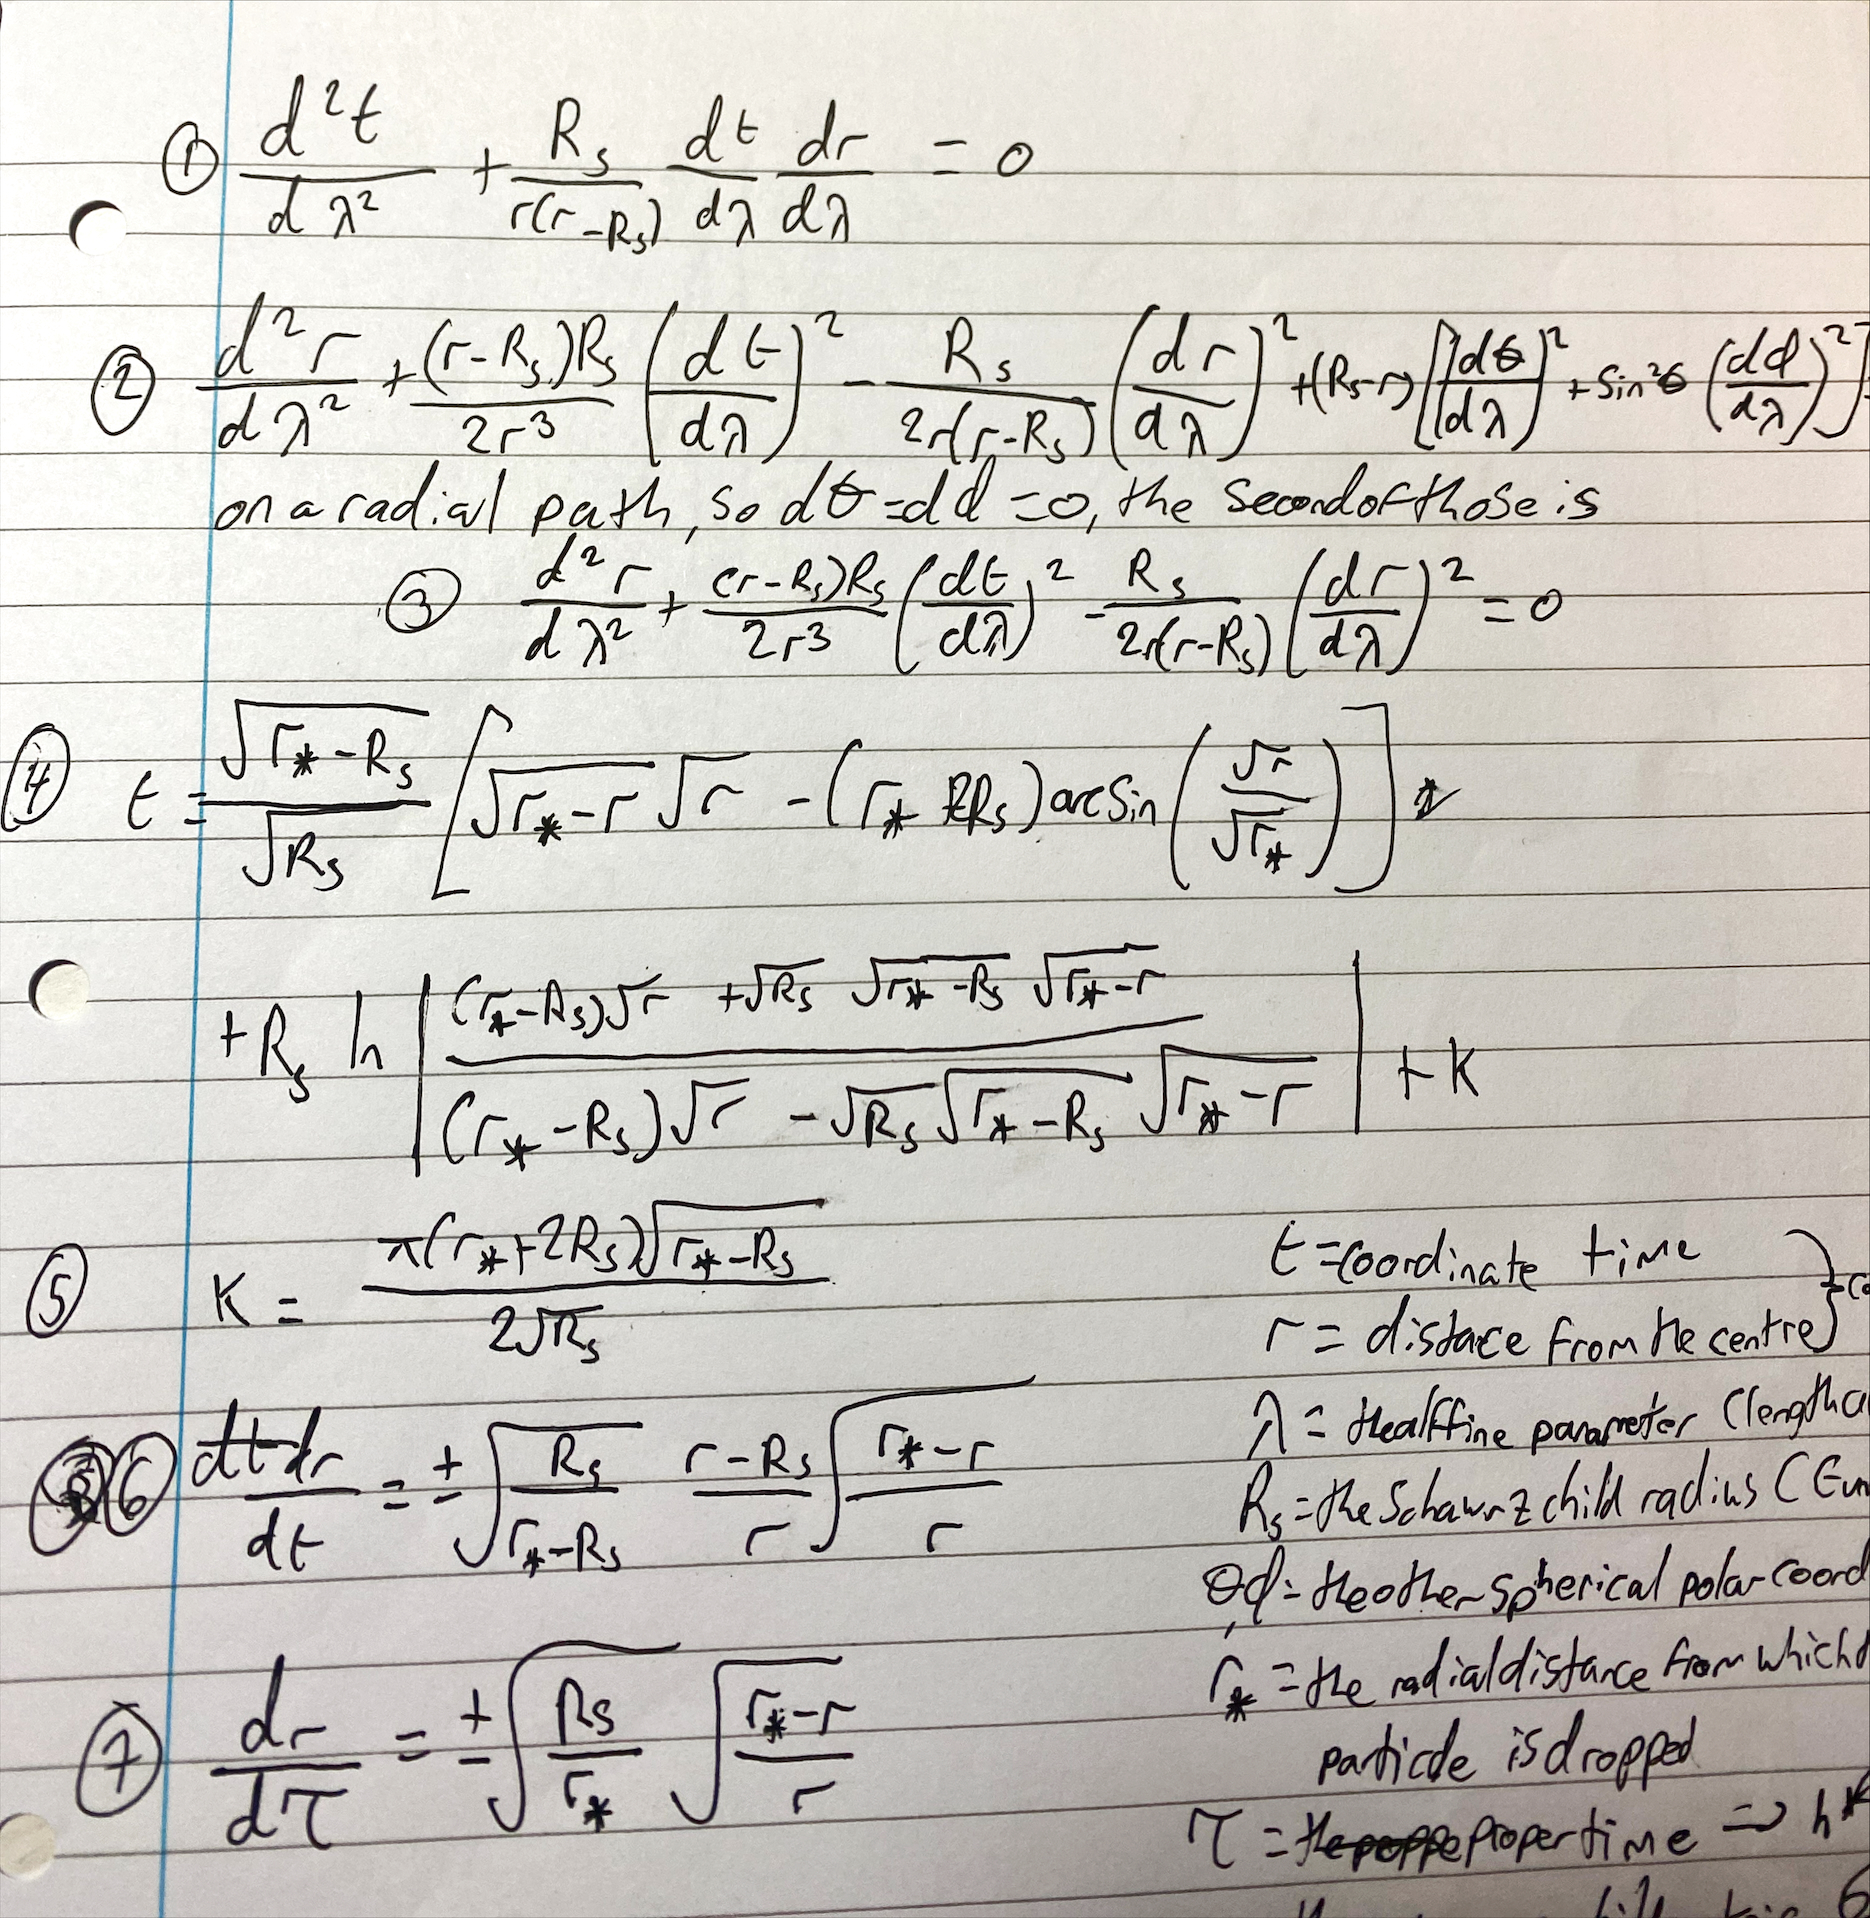
\includegraphics[width=0.25\textwidth]{figures/daniel_working.jpeg}
                    \end{center}
                    \caption{A sample of Daniel's working out}
                    \label{fig:daniel_working}
                \end{figure}


                \pagebreak


                \textbf{Advantages:}
                \begin{itemize}
                    \item Very versatile. Paper and pen allows for great customisation in the layout of the work including diagrams and annotations, which allows the user to be able to do things the way they want to do.
                    \item Cheap and easy to use. Little equipment is required and there isn't a need to install anything. 
                    \item Writing things physically on paper usually results in the writer being able to remember it easier, which would help in remembering things when learning. 
                    \item To get effective with analytic methods you require a lot of practice, which develops core skills like manipulation of various equations to achieve a desired result.
                    \item Ability to get exact answers and relationships between objects and attributes. Computers can only approximate exact answers and being able to see the equations of what is happening can greatly aid intuition when tackling future problems.
                    \item Doing hard work to get to a result is rewarding and relaxing. Offloading a lot of that work to a computer would reduce the enjoyment from this process.
                \end{itemize}


                \textbf{Disadvantages:}
                \begin{itemize}
                    \item Difficult to organise. You can't save paper notes in a way that is easily shareable and easy to organise on a computer (other than scanning them as PDF files which can take a lot of time and my clients find annoying). It may also be hard to stay consistent with formatting due to how versatile it is, as seen in \autoref{fig:daniel_working}.
                    \item Getting accurate graphs beyond simple sketches is difficult. Performing numerical methods by hand is very time-consuming which decreases the amount of time that can be spent on doing actual work. 
                    \item Scope of problems that can be approached is limited. Not all systems can be solved using analytic methods and sometimes numerical methods are necessary, depending on how simple or complex you choose to make your model.
                    \item Some problems are much harder to approach as the effectiveness of analytic methods is dependent on your ability to manipulate and work with equations, as well as general mathematical ability. Human's also make mistakes and are far less consistent than a computer at doing the same or similar calculations repeatedly.
                \end{itemize}

            \subsubsection{Desmos}

                % Desmos FIG
                \begin{figure}[!ht]
                    \begin{center}
                        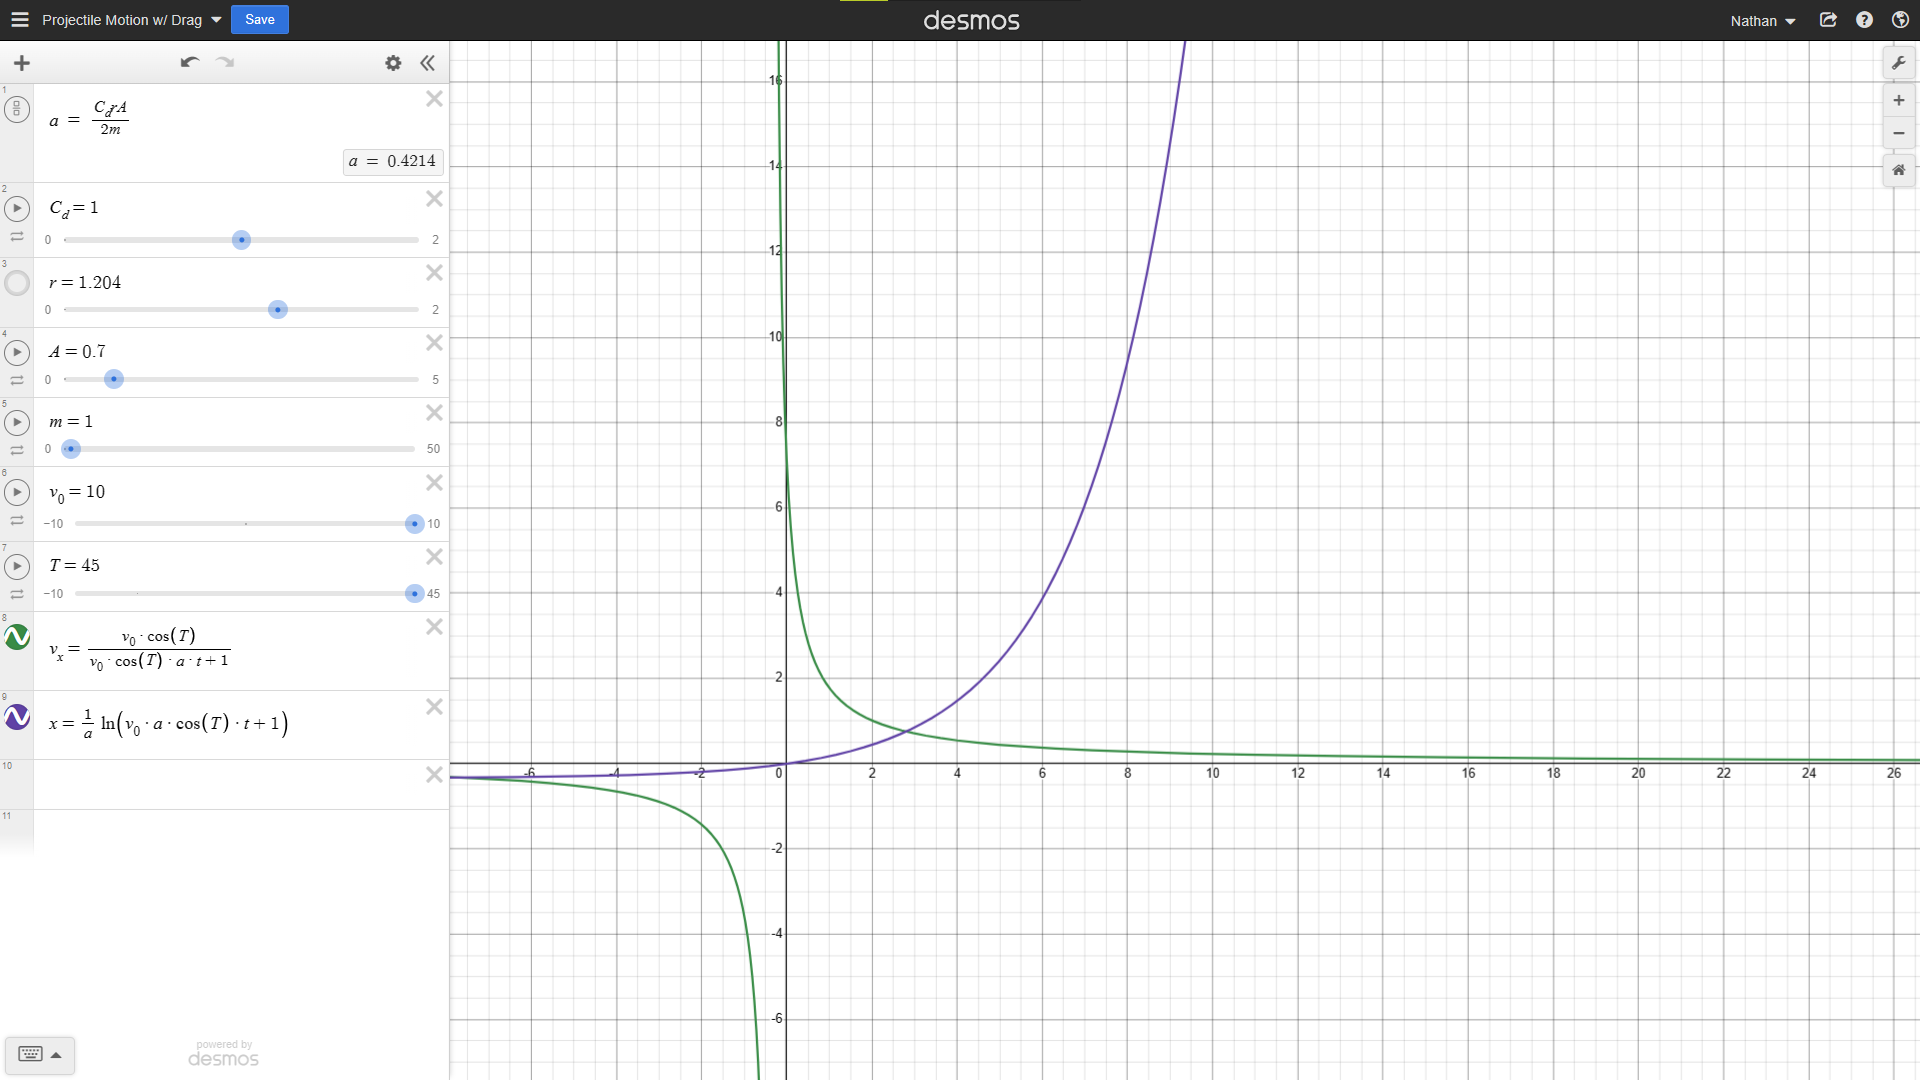
\includegraphics[width=.5\textwidth]{figures/desmos.png}
                    \end{center}
                    \caption{Desmos graphing software}
                    \label{fig:desmos}
                \end{figure}


                In \autoref{fig:desmos} below, Desmos has been used in order to see how attributes of an object change (specifically the $x$ position and velocity with respect to time of an object experiencing drag). Desmos is great in order to aid intuition and view general trends, however you still need to work through equations in order to have something to graph, and Desmos won't give exact values for solutions, but the final visualisations are still very useful. 

                The simplicity of Desmos allows it to be very versatile, but that also means its more of a jack-of-all-trades and master of none, so it wouldn't be very good for a more specialised application (like the ones being considered).


                \pagebreak
                \textbf{Advantages:}
                \begin{itemize}
                    \item Desmos is a very versatile software which means that it can be used for a wide variety of problems. 
                    \item Free and easy to use. Desmos can be accessed by anyone with a computer or mobile device by going to \href{https://www.desmos.com/calculator}{their website}, or by downloading the mobile app.
                    \item Very customisable. Desmos allows for labels within the equation space, as well as changing the names of the labels on the axes. Which allows for some form of documentation within the graphs. The colours and line style are also changeable.
                    \item Easy to share and work on on multiple devices. After you make an account, you are able to save graphs that you've done and access them on whatever device you're signed in on. Graphs can also be shared with links once they're saved which allows for collaboration on projects.
                    \item As of quite recently, Desmos has released a beta for a 3D graphing mode, which is great for modelling some events happening in 3D, such as the trajectory of an object given some initial conditions.
                \end{itemize}


                \textbf{Disadvantages:}
                \begin{itemize}
                    \item The versatility of Desmos means that in the case of a more specialised system with specific needs, it would be more beneficial to create custom software for that specific system. However, Desmos still manages to cover a wide variety of problems, just not in a lot of depth.
                    \item The accuracy of Desmos is not very customisable, usually giving answers to two or three decimal places, and it is only able to give exact answers in some circumstances (values are usually given in terms of $\pi$ when working with trigonometric functions).
                    \item Circuits diagrams often end up messy and obviously not functional as they are on a piece of paper.
                \end{itemize}



            % do another one later
            
            \subsubsection{Online Circuit Builder}
                I searched for some online JavaScript based circuit builders and I found this \href{https://www.falstad.com/circuit/}{Circuit Simulator Applet}. Although none of my clients have used this before, and I don't personally have a lot of experience with it, I can see that there are a lot of good features in this solution. The use of circuit symbols instead of renders of components allows students to familiarise themselves with them, as when actually drawing out circuit diagrams that's what they would use. Furthermore, as circuits get more and more complex and components get smaller, it may not even be practical or useful to look at a real life version of the circuit. 


                % Circuit Builder SS FIG
                \begin{figure}[!ht]
                    \begin{center}
                        \includegraphics[width=.5\textwidth]{figures/circuit_builder.png}
                    \end{center}
                    \caption{A simple circuit made on the circuit builder}
                    \label{fig:circuit_builder_ss1}
                \end{figure}


                % Circuit Builder SS2 FIG
                \begin{figure}[!ht]
                    \begin{center}
                        \includegraphics[width=.5\textwidth]{figures/circuit_graphs.png}
                    \end{center}
                    \caption{Graphs of attributes changing with respect to time and each other}
                    \label{fig:circuit_builder_ss2}
                \end{figure}


                \textbf{Advantages:}
                \begin{itemize}
                    \item The use of standard circuit symbols, which are 2D and quite simple shapes, instead of renders or images of actual components makes the program more efficient and increases performance, as no advanced rendering is necessary. 
                    \item Charge flow indicators in the form of yellow circles that represent electrons help visualise the flow of charge around a circuit for students. 
                    \item Including colour indicators do distinguish between places with negative and positive potential difference adds another level of interaction for the user, and this is something that could be quite hard to visualise and notice even with a real life version of the circuit available.
                    \item The simulation can be freely paused and unpaused in order to be able to see how a circuit appears at a specific point in time, which would be difficult with a real life version. 
                    \item The ability to plot real time graphs akin to an oscilloscope is as useful as having a real life oscilloscope, which is great when used to see how attributes change with respect to time and each other. See \autoref{fig:circuit_builder_ss2}.
                    \item The ability to export and import circuit arrangements is very useful as it allows for easier collaboration.
                \end{itemize}


                \textbf{Disadvantages:}
                \begin{itemize}
                    \item Although it contains a myriad of different components and pre-made circuits, some "features" are missing. For example, you can't set the internal resistance of a cell, and you also can't choose custom wires where you can alter the resistivity and length more precisely, which would make the simulation more accurate.
                    \item I found the system for placing new components in to be quite clunky and frustrating to get used to. Drawing the components is a good system, but the way it was implemented felt annoying to place in new components, it felt like you had to already know where you want to place components beforehand, which limits the freedom the user has to experiment with new arrangements. 
                \end{itemize}


        \pagebreak
        
        \subsection{Success Criteria of the Proposed System}
            This is a table of what the essential criteria for the solution are.

            % Essential Success Criteria TBL
            \begin{table}[!ht]
                \begin{center}
                \footnotesize
                \begin{tabular}{|l|m{187pt}|m{188pt}|l|}
                \hline
                ID & Feature & Justification & Ref. \\ \hline
                A1 & Model electric circuits \textbf{accurately} & This is the main purpose of the system and is something many of the stakeholders said they struggled with. & 1.5 \\ \hline
                A2 & Be able to handle \textbf{10 or fewer} components in a single circuit (excluding multimeters and wires). This requirement will be tested on my specific device, and possible on others if I get the access to them. & It is very uncommon for circuits studied at GCSE and A-Level to exceed 10 components, and as most of my clients study at that level I felt this number was appropriate. & 1.4 \\ \hline
                A3 & Have support for \textbf{at least} the following components: cell, wire, filament bulb, resistor, multimeter, switch. Each should have respective attributed be customisable (e.g. resistivity for wire, E.M.F. for cell) & This comes from analysis of common circuits seen at GCSE and A-Level circuits, which most commonly make use of these components. & 1.4 \\ \hline
                A4 & Have general attributes of the circuit displayed, such as total resistance, current, potential difference, and electro-motive forces & These are all useful attributes to know about a circuit when analysing it. &  \\ \hline
                A5 & Have a "snapshot" button that would be able to log attributes of all components at the time of the button press. This data could then be exported to a CSV file or similar for independent analysis by the user. & Allowing the user to easily collect data on components would make it easier for them to perform analysis on circuits and practice core skills that are a part of doing a practical at A-Level or GCSE. Building up these skills could allow for working with more complex systems to be easier. & 1.4 \\ \hline
                A6 & An intuitive way to add components to a circuit, most likely being able to drag components onto the main stage using the mouse. & This way of interaction seems like the most intuitive way of adding new components. This would allow the user to easily interact with the software and be able to spend more time on learning the content rather than learning how to use the software. & 1.4 \\ \hline
                A7 & \textbf{Charge flow indicators} to visualised charge flow around a circuit. Toggle between electron flow, conventional current, and off. & A concept that comes up in A-Level quite frequently is the conservation of charge and the actual movement of electrons and their interactions with circuit components. This feature would make it very easy to see how the electrons actually move about in the circuit, and make ideas like Kirchoff's Laws much easier to understand. & 1.4 \\ \hline
                A8 & Nameable components, for easier management. & If working on more complicated circuits, a way to be able to label components and then search for them would be very beneficial, rather than "component 1", "component 2", and so on, especially for my client Hugo who often works on complex electrical systems. & 1.4 \\ \hline
                \end{tabular}
                \end{center}
                \caption{Essential success criteria}
                \label{tbl:essential_succ_crit}
            \end{table}


            \pagebreak

            Here is a table of optional criteria for the solution, that would still benefit the users but aren't essential for it to be deemed functional and are mostly quality of life features.
            
            % Optional Success Criteria TBL
            \begin{table}[!ht]
                \begin{center}
                \footnotesize
                \begin{tabular}{|l|m{200pt}|m{200pt}|}
                \hline
                ID & Feature & Justification \\ \hline
                B1 & Be able to handle multiple (two or more) separate circuits running simultaneously. & This feature could be useful when studying more complex electrical systems, however it is more of a way to measure the performance and efficiency of the program, and this is a good target to work towards. \\ \hline
                B2 & Have the snapshot button be more customisable, with snapshots possible occurring automatically after a given time period. Could also have the snapshot button only take in certain attributes of certain components rather than all of them. & This feature would allow for easier monitoring of data as well as not having to take in all of the data, which could be a lot if the circuit is complex enough. \\ \hline
                B3 & Include customisable themes and/or accessibility features such as accounting for different types of colour blindness. & In order to make my solution as accessible as possible to help as many students as possible, being able to change the colour scheme would be a very useful feature. \\ \hline
                B4 & Being able to export and import circuit arrangements. & This would allow for easier collaboration, also between students and teachers, which would help as it would be much easier to communicate ideas. \\ \hline
                B5 & Adding keyboard shortcuts & Keyboard shortcuts would heavily streamline the use of a software like this, especially as the user gets more and more accustomed to them over time, as is common in many scientific programs. \\ \hline
                \end{tabular}
                \end{center}
                \caption{Optional success criteria}
                \label{tbl:optional_succ_crit}
            \end{table}
        
        
        % \subsection{Data Source(s)}
        % \subsection{Volumetrics - Data Volumes}
        % \subsection{Analysis Data Dictionary}
        % \subsection{Data Flow Diagrams for Existing and Proposed System}


        \subsection{Justification of Chosen Solution}
            My proposed solution is to create a piece of software that functions as a electrical circuit builder allowing the user to place different components on a main board and then connect them using wires. Then the software would simulate what is happening at each component as well as allow those attributes to be viewed and logged by the user within the software. Circuits wouldn't be able to be edited while they are being simulated, as the two modes would be completely separate from each other.

            This solution would be very good as it would allow for a concept that a lot of students struggle with to be visualised. A lot of students do not have access to circuit components at home, and so trying to study circuits independently can be very challenging for some. A much larger proportion of students own a computer with a mouse and keyboard at their home, so a piece of software would be more accessible to most if not all students. Also, as education shifts more and more into digital, a way of collaborating on circuits through the internet (with just being able to send an exported file to another person) greatly aids student understanding and ability to learn.

        \subsection{Hardware and Software}
            The system will only require a computer with a working mouse and display to work properly, but the functionality for keyboard shortcuts is a possibility in the future. Regarding software, only the actual program is would be necessary, and distributing it to the end user would be a trivial task.

        \subsection{Limitations}
            I only have experience with GUI elements while using Python, however the complexity and amount of processing needed for the project may exceed the capabilities of Python. As such careful consideration into how features are implemented would have to be taken as I need the program to be as efficient as possible. 

        % \subsection{Entity-Relationship Models}
        % \subsection{Identification of Objects and Object Analysis Diagrams}

    \section{Overall System Design}
            I decided to split the system into three sections: project, simulating, building. Within the software, the user will initialise a "project" in a directory. The program will frequently refer to a "source directory", which will be the user's program files by default. This source directory will be configurable by the user, but there is no guarantee that the user changing things on their own won't break some of the functionality.

            % Overall Hierarchy Diagram FRST
            \begin{center}
                \footnotesize
                \begin{forest}
                    for tree={
                        align=center,
                        font=\sffamily,
                    edge+={thick, -{Stealth[]}},
                    l sep'+=10pt,
                    fork sep'=10pt,
                    },
                    forked edges,
                    if level=0{
                        inner xsep=0pt,
                        tikz={\draw [thick] (.children first) -- (.children last);}
                        }{},
                        [Circuit Builder
                            [Project/File Management
                                [Initialising
                                    [Choose to\\make new or\\open file
                                        [Importing\\all data and\\rendering]
                                        [Initialising\\necessary files]
                                    ]
                                    [Choose working\\directory]
                                ]
                                [Exporting
                                    [Data]
                                    [Project/Circuit\\arrangement]
                                ]
                            ]
                            [Simulating
                                [Updating\\attributes of\\components
                                    [Rendering\\updates]
                                    [Storing data]
                                ]
                                [Rendering\\graphs]
                            ]
                            [Building
                                [Placing\\components
                                    [Choosing\\component]
                                    [Choosing\\location]
                                ]
                                [Editing\\attributes
                                    [Menu\\interactions]
                                ]
                            ]
                        ]
                    \end{forest}
            \end{center}
                
            Each cycle will be taken on individually. I'll fix the formatting later.
            
    \section{Cycle 1: Project and File Management}
        Here is the hierarchy diagram from the previous section. It considers two tasks, exporting and initialising.

        % C1 Hierarchy Diagram FRST
        \begin{center}
            \footnotesize
            \begin{forest}
                for tree={
                    align=center,
                    font=\sffamily,
                edge+={thick, -{Stealth[]}},
                l sep'+=10pt,
                fork sep'=10pt,
                },
                forked edges,
                if level=0{
                    inner xsep=0pt,
                    tikz={\draw [thick] (.children first) -- (.children last);}
                    }{},
                    [Project and File Management
                        [Opening projects
                            [Initialising\\new projects
                                [Making sure\\all relevant\\files are present]
                                [Choosing\\working directory]
                                [Initialising all\\the files]
                            ]
                            [Opening existing\\projects
                                [Choosing\\working directory]
                                [Verifying files]
                            ]
                        ]
                        [Exporting circuit\\arrangements
                            [Choosing\\destination]
                            [Compressing\\and exporting]
                        ]
                    ]
            \end{forest}
        \end{center}

        \subsection{Brief Outline}
            In this cycle I will create the programming for some interactive UI that will allow the user to initialise or open a project as well as export the project so that it would be able to be accessed by other people.


            \subsubsection{Success Criteria}
                These are the success criteria that are going to be used. ID beginning with "X" indicates that it was specifically added for this cycle.

                % Success Criteria C1 TBL
                \begin{table}[!ht]
                    \begin{center}
                    \begin{tabular}{m{16pt}m{0.8\textwidth}}
                    ID & Feature \\ \hline
                    B4 & Being able to export and import circuit arrangements. \\ 
                    X1 & Only open directories that include all relevant files, raising an exception when this isn't met. \\ 
                    X2 & Copy relevant files from the source directory in order to initialise a project. \\ 
                    X3 & Allow user to specify directory for exporting. \\ 
                    X4 & Compress exported files intuitively. \\ 
                    \end{tabular}
                \end{center}
                \caption{Success criteria for cycle 1}
                \label{tbl:succ_crit_c1}
                \end{table}


        \subsection{Design}
            \subsubsection{User Interface}
                Will insert annotated drawings later.

            \subsubsection{Data Structures}

                % Data structures C1 TBL
                \begin{table}[!ht]
                    \begin{center}
                        \begin{tabular}{llm{0.5\textwidth}}
                        Name & Data Type/Structure & Data \\ \hline
                        \verb|project_name| & String (var.) & Name of the project (will be used in displays and for organisational purposes) \\
                        \verb|working_dir| & String (var.) & The working directory of the project \\
                        \verb|source| & String (const.) & Where all the relevant files are initially stored \\
                        \verb|location| & String (var.) & Destination folder for exporting, inputted by user \\
                        \verb|permissions| & Bool (var.) & True if and only if the instance of the program has been run with administrator privileges. This limits the directories available.
                        \end{tabular}
                    \end{center}
                \caption{Data structures that will be used in cycle 1}
                \label{tbl:data_structs_c1}
                \end{table}


                The user may not always have permissions to save into/export into the directory they have selected. When doing file management using for example the file explorer on Windows 10, the operating system will handle telling the user that they have invalid permissions. However, when attempting operations on files with invalid permissions through a programming language such as Python, the error will be raised in the program. Due to this I have included a \verb|permissions| variable that checks whether the program has permissions to write to a given directory to prevent this.


                \pagebreak


            \subsubsection{Algorithms}


                I decided to plan some of my key algorithms for this cycle, namely the algorithms responsible for exporting files, initialising a project, and installing the program.


                % Exporting flow chart FIG
                \begin{figure}[!ht]
                \begin{center}
                    \includegraphics[width=.2\textwidth]{figures/algorithms/c1_export.png}
                \end{center}
                \caption{Flowchart for exporting a project}
                \label{fig:exporting_fc_c1}
                \end{figure}
                

                % Initialise project PC
                \begin{figure}[!ht]
                    \begin{minted}[linenos]{python}
    import os
    source = "Source directory here"
    procedure init_files(target)
        if target.permissions == False:
            raise PermissionError
        files = os.listdir(source)
        for f in files:
            f.copy(target)
    endprocedure
                    \end{minted}
                    \caption{Pseudocode to copy initial project files to a folder}
                    \label{pc:copy_to_folder_ps_c1}
                \end{figure}


                The file running the procedure above will need to be in the same location as the folder it is copying from. To make the file easier to access, the program could make a shortcut to this file and add it to the desktop for the user.
                

                % Install main program PC
                \begin{figure}[!ht]
                \begin{minted}[linenos]{python}
    url = https://github.com/nathan-tat/cs_nea_2025/tree/main/code/software
    procedure install_software(target)
        if target.permissions == False:
            raise PermissionError
        
        download_from_github(url, target)
                \end{minted}
                \caption{Pseudocode to install the main program}
                \label{pc:install_software_ps_c1}
                \end{figure}


                The installer will copy files from a GitHub repository, where all the files necessary for the program to run will be stored, into a folder specified by the user on the user's computer. This folder will then be referred to as \verb|source| (see \autoref{tbl:data_structs_c1})


            \subsubsection{Test Data}
                Need to write up test data

        

        \subsection{Implementation}
            There are two files in this cycle, one for the installer and one for the opener of file projects and I will tackle them seperately.


            \subsubsection{Installer}
                The installer will copy files from a specified repository on GitHub, which will store all the necessary files for the program to run, into a folder specified by the user, which will then be referred to by the program as the source folder. 


                % InstallGUI Class Diagram FIG
                \begin{figure}[!ht]
                   \begin{center}
                    %    \includegraphics[width=.25\textwidth]{figures/install_gui_class_diagram.png}
                   \end{center}
                   \caption{Class diagram for the InstallGUI class}
                   \label{fig:installgui_class_diagram_c1}
                \end{figure}


                The buttons on the GUI element are attributes in the class which means I am able to access and edit their attributes within methods of the class. 

                In \autoref{snip:install_gui_init_sc_c1}, the position, size, and text of the individual UI elements have been initialised as well as some of the attributes of the main window.


                % Cancel and Browse buttons SC
                \begin{figure}[!ht]
                \begin{minted}[linenos]{python}
    def btn_cancel_command(self) -> None:
        """ Closes the UI window safely """
        print("Exiting...")
        root.destroy()

    def btn_browse_command(self) -> None:
        """ Allows the user to select a directory to 
        install the software into. """
        self.filepath = filedialog.askdirectory()
        self.lbl_welcome["text"] = self.filepath
        self.ent_dir["text"] = self.filepath
        self.btn_install["state"] = "active"
                \end{minted}
                \caption{Code for cancel and browse}
                \label{snip:cancel_and_browse_btns_sc_c1}
                \end{figure}


                In \autoref{snip:cancel_and_browse_btns_sc_c1}, the browse button will open a dialogue allowing the user to select a folder into which they would like to install the software.


                % Install btn SC
                \begin{figure}[!ht]
                \begin{minted}[linenos]{python}
    def btn_install_command(self) -> None:
        """ Installs the software to the given directory. Probably very not secure. """
        # set it equal to eachother <3
        if self.filepath != self.ent_dir["text"]:
            self.filepath = self.ent_dir["text"]
            
        # if not a real directory
        if not os.path.isdir(self.filepath):
            pass
        
        # do some fancy stuffs
        # like turning off some of the buttons
        self.btn_browse["state"] = "disabled"
        self.btn_cancel["state"] = "disabled"
        self.btn_install["state"] = "disabled"
        
        self.lbl_welcome["text"] = "Please wait... Downloading..."
        
        
        # this probably works
        try:
            install_requirements(REQ)
            download_from_github(self.filepath)
        except:
            self.lbl_welcome["text"] = "something bad happened"
        else:
            self.lbl_welcome["text"] = "Thank you. Downloaded. "
        
        self.btn_browse["state"] = "active"
        self.btn_cancel["state"] = "active"
        self.btn_install["state"] = "active"
                \end{minted}
                \caption{Code for install button}
                \label{snip:install_btn_sc_c1}
                \end{figure}


                This button will disable all the buttons while the software is installing. I think I would like to add a progress indicator in the future.


                % InstallGUI class init SC
                \begin{figure}[!ht]
                \begin{minted}[linenos]{python}
class InstallGUI:
    def __init__(self, root):
        #setting title
        root.title("Installer")
        #setting window size
        w = 305
        h = 160
        sw = root.winfo_screenwidth()
        sh = root.winfo_screenheight()
        alignstr = '%dx%d+%d+%d' % (w, h, (sw - w) / 2, (sh - h) / 2)
        root.geometry(alignstr)
        root.resizable(width=False, height=False)

        self.btn_cancel = tk.Button(root)
        self.btn_cancel["text"] = "Cancel"
        self.btn_cancel.place(x=20,y=110,width=70,height=25)
        self.btn_cancel["command"] = self.btn_cancel_command

        self.btn_install = tk.Button(root)
        self.btn_install["text"] = "Install"
        self.btn_install.place(x=210,y=110,width=70,height=25)
        self.btn_install["command"] = self.btn_install_command
        self.btn_install["state"] = "disabled"

        self.btn_browse = tk.Button(root)
        self.btn_browse["text"] = "Browse"
        self.btn_browse.place(x=200,y=60,width=79,height=30)
        self.btn_browse["command"] = self.btn_browse_command

        self.ent_dir = tk.Entry(root)
        self.ent_dir["justify"] = "left"
        self.ent_dir["text"] = "C:\\Program Files\\"
        self.ent_dir.place(x=20,y=60,width=183,height=30)

        self.lbl_welcome = tk.Label(root)
        self.lbl_welcome["justify"] = "center"
        self.lbl_welcome["text"] = "this is the installer"
        self.lbl_welcome.place(x=20,y=20,width=170,height=30)
        
        self.filepath = None
                \end{minted}
                \caption{Initialising method for the InstallGUI class}
                \label{snip:install_gui_init_sc_c1}
                \end{figure}


                % Installer GUI evidence FIG
                \begin{figure}[!ht]
                   \begin{center}
                    %    \includegraphics[width=.5\textwidth]{figures/installer1.png}
                   \end{center}
                   \caption{Installer in action}
                   \label{fig:installer_gui_ss1_c1}
                \end{figure}


                The directory doesn't show on the entry box so I need to fix that (I'll take screenshots later).
        \subsubsection{Opener}
                This code isnt finished yet.




    %     \subsection{Annotated Listing of the Program(s)}
    %     \subsection{Annotated "Design Views" showing details of application-generated forms, reports, queries, buttons, cross tabulations, etc.}
    %     \subsection{Procedure and Variable List}
    %     \subsection{Testing to inform development - Testing at each stage}
    %     \subsection{Re-Testing}

    % % Join with previous section 
    % \section{Testing}
    %     \subsection{Test Plan}
    %     \subsection{Test Data}
    %     \subsection{Areas to Test}
    %     \subsection{Tables}
    %     \subsection{Justification of Data Selection}
    %     \subsection{Evidence of Testing}
    %     \subsection{Program Listing}
    
    % \section{Evaluation}
    %     \subsection{Comparison of Performance of your System against Success Criteria}
    %     \subsection{Analysis of User Feedback}
    %     \subsection{Evaluation of Usability Features}
    %     \subsection{Maintenance Issues and Limitations of the Product}
    %     \subsection{Improvements and Possible Extensions}
        

\end{document}